\documentclass[twoside, final]{hcmut_report}
% \usepackage{codespace}
% Configuration
\upperuniname{ĐẠI HỌC QUỐC GIA THÀNH PHỐ HỒ CHÍ MINH}
\uniname{TRƯỜNG ĐẠI HỌC BÁCH KHOA}
\deptname{KHOA KHOA HỌC VÀ KỸ THUẬT MÁY TÍNH}

\coursename{XÁC SUẤT VÀ THỐNG KÊ}
\reporttype{BÁO CÁO BÀI TẬP LỚN}
\title{PHÂN TÍCH GIÁ TRỊ TỔNG ĐƠN HÀNG Ở MỘT CỬA HÀNG ĐIỆN TỬ}
\advisor{
    TS. Phan Thị Hường
}
\student{
    Trần Điền Minh          ,   2312116
    Phan Thanh Sơn          ,   2312975
    Nguyễn Hoàng Anh Thắng  ,   2313185
    Huỳnh Văn Lợi           ,   2311974
    Cao Chí Nguyên          ,   2312331
    Nguyễn Hữu Thịnh        ,   2313292
}

\begin{document}
\begin{titlepage}
    \coverpage
    \newpage
    \begin{center}
        \small \bfseries 
        BÁO CÁO PHÂN CÔNG NHIỆM VỤ VÀ KẾT QUẢ THỰC HIỆN ĐỀ TÀI         
        
        NHÓM: 10 -- LỚP: TN01 -- HỌC KỲ: 241 -- MÔN: XÁC SUẤT VÀ THỐNG KÊ   
    \renewcommand{\arraystretch}{1.2}
    \begin{table}[h!]
        \centering
        \resizebox{\textwidth}{!}{%
        \begin{tabular}{|c|l|c|l|c|c|}
            \hline
            \textbf{STT} & \textbf{Họ và tên}         & \textbf{MSSV}   & \textbf{Nhiệm vụ}                             & \textbf{Đóng góp} & \textbf{Điểm chia $\pm 2$} \\ \hline
            1            & Trần Điền Minh            & 2312116         & Hồi quy đa bội                                 & 100 \% & 0 \\ \hline
            2            & Phan Thanh Sơn            & 2312975         & Hồi quy đa bội                                 & 100 \% & 0 \\ \hline
            3            & Nguyễn Hoàng Anh Thắng    & 2313185         & Anova hai nhân tố                              & 100 \% & 0 \\ \hline
            4            & Huỳnh Văn Lợi             & 2311974         & Anova một nhân tố                              & 100 \% & 0 \\ \hline
            5            & Cao Chí Nguyên            & 2312331         & Thống kê mô tả                       & 100 \% & 0 \\ \hline
            6            & Nguyễn Hữu Thịnh          & 2313292         & Tiền xử lí số liệu                   & 100 \% & 0 \\ \hline
        \end{tabular}
        }        
    \end{table}
\end{center}
    \newpage
    \tableofcontents
    \newpage
\end{titlepage}

\setcounter{page}{1}
\pagestyle{empty}

\pagestyle{fancy}
\pagebreak
\section{Tổng quan dữ liệu}
\subsection{Mô tả dữ liệu}
Tập dữ liệu được cung cấp trong BTL chứa thông tin về một cửa hàng điện tử trực tuyến. Cửa hàng có ba kho hàng hóa để giao hàng cho khách hàng. Dựa vào dữ liệu đã cho để tìm mối quan hệ giữa các biến, từ đó xây dựng mô hình giúp hiểu rõ những yếu tố ảnh hưởng đến giá trị của tổng đơn hàng.

\begin{itemize}
    \item Tiêu đề: Transactional Retail Dataset of Electronics Store
    \item Thông tin nguồn:
        \begin{itemize}
            \item Tác giả: SHAHRAYAR
            \item Thời điểm công bố dữ liệu: 3 năm trước
        \end{itemize}
    \item Giá trị quan trắc: 500
    \item Số lượng biến: 16
\end{itemize}
Trong bài tập lớn này, nhóm đã quyết định sử dụng file \textbf{dirty\_data.csv} để làm dữ liệu cho việc xây dựng các mô hình thống kê.
\subsection{Mô tả biến}
Dữ liệu dưới đây được thu thập và tổ chức nhằm mục đích hỗ trợ quá trình phân tích và quản lý đơn hàng trong hệ thống thương mại điện tử. Đây là tập hợp các thông tin chi tiết liên quan đến đơn đặt hàng, khách hàng, sản phẩm, và các yếu tố khác có liên quan.

Các biến được chia thành hai dạng tương ứng:
\begin{itemize}
    \item \textbf{7 biến phân loại:} order\_id, customer\_id, nearest\_warehouse, season, is\_expedited\_delivery, latest\_customer\_review, is\_happy\_customer.
    \item \textbf{6 biến liên tục:} order\_price, delivery\_charges, customer\_lat, customer\_long, coupon\_discount, order\_total, distance\_to\_nearest\_warehouse. 
\end{itemize}

Mỗi biến trong bảng dữ liệu đều được mô tả một cách cụ thể, bao gồm: Tên biến, loại dữ liệu, đơn vị đo lường (nếu có), và ý nghĩa của biến.
Các thông tin này giúp làm rõ bản chất và vai trò của từng trường dữ liệu trong hệ thống. Dữ liệu này không chỉ hỗ trợ phân tích các xu hướng mua hàng mà còn cung cấp các thông tin quan trọng để dự đoán nhu cầu, tối ưu hóa chi phí vận hành và cải thiện trải nghiệm khách hàng. Bảng dưới đây trình bày chi tiết từng biến, được tổ chức theo từng nhóm thông tin cụ thể, giúp người đọc dễ dàng tiếp cận và hiểu rõ hơn về dữ liệu được sử dụng.

\vspace{0.5cm}

% Row 1
\noindent
\begin{minipage}[t]{0.48\textwidth}
\begin{mainbox}{Biến 1: order\_id}{1}
    \textbf{Loại dữ liệu:} Chuỗi kí tự \\
    \textbf{Đơn vị:} (Trống) \\
    \textbf{Mô tả:} Một ID duy nhất cho mỗi đơn hàng.
\end{mainbox}
\end{minipage}
\hfill
\begin{minipage}[t]{0.48\textwidth}
\begin{mainbox}{Biến 2: customer\_id}{1}
    \textbf{Loại dữ liệu:} Chuỗi kí tự \\
    \textbf{Đơn vị:} (Trống) \\
    \textbf{Mô tả:} Một ID duy nhất cho mỗi khách hàng.
\end{mainbox}
\end{minipage}

\vspace{0.5cm}

% Row 2
\noindent
\begin{minipage}[t]{0.48\textwidth}
\begin{mainbox}{Biến 3: date}{2}
    \textbf{Loại dữ liệu:} Chuỗi kí tự \\
    \textbf{Đơn vị:} (Trống) \\
    \textbf{Mô tả:} Ngày đặt hàng, được đưa ra ở định dạng YYYY-MM-DD.
\end{mainbox}
\end{minipage}
\hfill
\begin{minipage}[t]{0.48\textwidth}
\begin{mainbox}{Biến 4: nearest\_warehouse}{2}
    \textbf{Loại dữ liệu:} Chuỗi kí tự \\
    \textbf{Đơn vị:} (Trống) \\
    \textbf{Mô tả:} Một chuỗi biểu thị tên của kho hàng gần nhất với khách hàng.
\end{mainbox}
\end{minipage}

\vspace{0.5cm}

% Row 3
\noindent
\begin{minipage}[t]{0.48\textwidth}
\begin{mainbox}{Biến 5: shopping\_cart}{3}
    \textbf{Loại dữ liệu:} Chuỗi kí tự \\
    \textbf{Đơn vị:} (Trống) \\
    \textbf{Mô tả:} Một danh sách các bộ đại diện cho các hạng mục trong đơn hàng: phần tử đầu tiên của bộ dữ liệu là mục được sắp xếp và phần tử thứ hai là số lượng đặt hàng cho mặt hàng đó.
\end{mainbox}
\end{minipage}
\hfill
\begin{minipage}[t]{0.48\textwidth}
\begin{mainbox}{Biến 6: order\_price}{3}
    \textbf{Loại dữ liệu:} \(x \in (0; +\infty)\) \\
    \textbf{Đơn vị:} USD \\
    \textbf{Mô tả:} Một số biểu thị giá đặt hàng bằng USD. Giá đặt hàng là giá của các mặt hàng trước khi có bất kỳ khoản giảm giá và/hoặc phí giao hàng nào được áp dụng.
\end{mainbox}
\end{minipage}

\vspace{0.5cm}

% Row 4
\noindent
\begin{minipage}[t]{0.48\textwidth}
\begin{mainbox}{Biến 7: delivery\_charges}{4}
    \textbf{Loại dữ liệu:} \(y \in (0; +\infty)\) \\
    \textbf{Đơn vị:} USD \\
    \textbf{Mô tả:} Một số thể hiện phí giao hàng của đơn hàng.
\end{mainbox}
\end{minipage}
\hfill
\begin{minipage}[t]{0.48\textwidth}
\begin{mainbox}{Biến 8: customer\_lat}{4}
    \textbf{Loại dữ liệu:} \(z \in (-90; 90)\) \\
    \textbf{Đơn vị:} Độ \\
    \textbf{Mô tả:} Vĩ độ vị trí của khách hàng.
\end{mainbox}
\end{minipage}

\vspace{0.5cm}

% Row 5
\noindent
\begin{minipage}[t]{0.48\textwidth}
\begin{mainbox}{Biến 9: customer\_long}{5}
    \textbf{Loại dữ liệu:} \(t \in (-180; 180)\) \\
    \textbf{Đơn vị:} Độ \\
    \textbf{Mô tả:} Kinh độ vị trí của khách hàng.
\end{mainbox}
\end{minipage}
\hfill
\begin{minipage}[t]{0.48\textwidth}
\begin{mainbox}{Biến 10: coupon\_discount}{5}
    \textbf{Loại dữ liệu:} \(m \in \mathbb{N}, 0 \leq m \leq 100\) \\
    \textbf{Đơn vị:} \% \\
    \textbf{Mô tả:} Một số nguyên biểu thị phần trăm giảm giá được áp dụng cho đơn giá.
\end{mainbox}
\end{minipage}

\vspace{0.5cm}

% Row 6
\noindent
\begin{minipage}[t]{0.48\textwidth}
\begin{mainbox}{Biến 11: order\_total}{6}
    \textbf{Loại dữ liệu:} \(n \in (0; +\infty), n \leq x\) \\
    \textbf{Đơn vị:} USD \\
    \textbf{Mô tả:} Một số biểu thị tổng giá tiền đơn đặt hàng bằng USD, giảm giá và/hoặc phí giao hàng đã được áp dụng.
\end{mainbox}
\end{minipage}
\hfill
\begin{minipage}[t]{0.48\textwidth}
\begin{mainbox}{Biến 12: season}{6}
    \textbf{Loại dữ liệu:} Chuỗi kí tự \\
    \textbf{Đơn vị:} (Trống) \\
    \textbf{Mô tả:} Một chuỗi biểu thị mùa mà đơn hàng được đặt.
\end{mainbox}
\end{minipage}

\vspace{0.5cm}

% Row 7
\noindent
\begin{minipage}[t]{0.48\textwidth}
\begin{mainbox}{Biến 13: is\_expedited\_delivery}{7}
    \textbf{Loại dữ liệu:} \(t = \text{TRUE}\) (có), \(t = \text{FALSE}\) (không) \\
    \textbf{Đơn vị:} (Trống) \\
    \textbf{Mô tả:} Một hàm nhị phân biểu thị liệu khách hàng có yêu cầu giao hàng nhanh hay không.
\end{mainbox}
\end{minipage}
\hfill
\begin{minipage}[t]{0.48\textwidth}
\begin{mainbox}{Biến 14: distance\_to\_nearest\_warehouse}{7}
    \textbf{Loại dữ liệu:} \(r \in (0; +\infty)\) \\
    \textbf{Đơn vị:} km \\
    \textbf{Mô tả:} Một số biểu thị khoảng cách vòng cung, tính bằng km, giữa khách hàng và kho hàng gần nhất với họ.
\end{mainbox}
\end{minipage}

\vspace{0.5cm}

% Row 8
\noindent
\begin{minipage}[t]{0.48\textwidth}
\begin{mainbox}{Biến 15: latest\_customer\_review}{8}
    \textbf{Loại dữ liệu:} Chuỗi kí tự \\
    \textbf{Đơn vị:} (Trống) \\
    \textbf{Mô tả:} Một chuỗi đại diện cho đánh giá mới nhất của khách hàng về đơn hàng gần đây nhất của họ.
\end{mainbox}
\end{minipage}
\hfill
\begin{minipage}[t]{0.48\textwidth}
\begin{mainbox}{Biến 16: is\_happy\_customer}{8}
    \textbf{Loại dữ liệu:} \(q = \text{TRUE}\) (có), \(q = \text{FALSE}\) (không) \\
    \textbf{Đơn vị:} (Trống) \\
    \textbf{Mô tả:} Một hàm nhị phân biểu thị liệu khách hàng có hài lòng hay không? Hoặc gặp vấn đề với đơn hàng gần đây nhất của họ.
\end{mainbox}
\end{minipage}
\section{Kiến thức nền}\label{Kien thuc nen}
\subsection{Thống kê mô tả}
Phương pháp thống kê mô tả (descriptive statistics) là một phương pháp trong khoa học thống kê được sử dụng để mô tả và tóm tắt các dữ liệu một cách đơn giản và dễ hiểu. Phương pháp này giúp chúng ta hiểu thông tin cơ bản về các biến trong dữ liệu mà không cần đưa ra các phán đoán hay suy luận về mối quan hệ giữa các biến. Các phương pháp thống kê mô tả thường bao gồm các đại lượng thống kê như \textbf{giá trị trung bình, phương sai, độ lệch chuẩn, phân vị, tỉ lệ phần trăm, đồ thị và biểu đồ}. Các đại lượng này giúp chúng ta hiểu về trung tâm, phân tán và hình dạng của dữ liệu.
\subsection{Thống kê suy diễn}
Trong bài tập lớn này, nhóm có vận dụng những kiến thức được học trên lớp như xây dựng khoảng tin cậy, kiểm định giả thuyết, định lý giới hạn trung tâm, v.v... Tuy nhiên, 
\subsubsection{Phân tích phương sai 2 nhân tố}
Phân tích phương sai 2 nhân tố (Two-Way ANOVA) là một phương pháp thống kê được sử dụng để kiểm tra sự ảnh hưởng của hai yếu tố (hay còn gọi là biến độc lập) đến một biến phụ thuộc (biến kết quả), cũng như mối quan hệ tương tác giữa chúng.

Giả sử có hai yếu tố \textit{A} và \textit{B}, với các mức độ tương ứng là a và b. Mô hình phân tích phương sai 2 nhân tố được xây dựng như sau:
\[
Y_{ijk} = \mu + \alpha_i + \beta_j + (\alpha \beta)_{ij} + \epsilon_{ijk}
\]
Trong đó:
\begin{itemize}
  \item \( Y_{ijk} \): giá trị quan sát thứ \( k \) của tổ hợp mức độ \( i \) của yếu tố \( A \) và mức độ \( j \) của yếu tố \( B \).
  \item \( \mu \): giá trị trung bình tổng thể.
  \item \( \alpha_i \): hiệu ứng của mức độ \( i \) của yếu tố \( A \).
  \item \( \beta_j \): hiệu ứng của mức độ \( j \) của yếu tố \( B \).
  \item \( (\alpha\beta)_{ij} \): hiệu ứng tương tác giữa yếu tố \( A \) và \( B \).
  \item \( \epsilon_{ijk} \): sai số ngẫu nhiên (residual).
\end{itemize}
\subsection{Hồi quy tuyến tính đa bội}
Hồi quy tuyến tính đa biến là một phương pháp thống kê được sử dụng để mô hình hóa mối quan hệ giữa một biến phụ thuộc (hay còn gọi là biến mục tiêu) và một hoặc nhiều biến độc lập (biến giải thích). Mục tiêu của hồi quy tuyến tính đa biến là dự đoán giá trị của biến phụ thuộc dựa trên các giá trị của các biến độc lập.

Mô hình hồi quy tuyến tính đa biến có dạng:

\[
Y = \beta_0 + \beta_1 X_1 + \beta_2 X_2 + \dots + \beta_p X_p + \epsilon
\]

Trong đó:
\begin{itemize}
  \item \(Y\) là biến phụ thuộc (biến mục tiêu).
  \item \(X_1, X_2, \dots, X_p\) là các biến độc lập (biến giải thích).
  \item \(\beta_0\) là hệ số chặn (intercept), đại diện cho giá trị của \(Y\) khi tất cả các biến độc lập đều bằng 0.
  \item \(\beta_1, \beta_2, \dots, \beta_p\) là các hệ số hồi quy (coefficient) đại diện cho mức độ tác động của mỗi biến độc lập đến biến phụ thuộc.
  \item \(\epsilon\) là sai số ngẫu nhiên (error term), thể hiện phần sai khác giữa giá trị thực tế của \(Y\) và giá trị dự đoán.
\end{itemize}

\textbf{Phương pháp bình phương tối thiểu (Ordinary Least Squares - OLS)}: Là phương pháp phổ biến nhất để ước lượng các hệ số \(\beta\) trong hồi quy tuyến tính. Mục tiêu là tìm giá trị của \(\beta\) sao cho tổng bình phương sai số (\(\epsilon\)) là nhỏ nhất.
  
\[
\text{Minimize } \sum_{i=1}^{n} (Y_i - (\beta_0 + \beta_1 X_{i1} + \dots + \beta_p X_{ip}))^2
\]

Sau khi ước lượng các hệ số \(\beta\), chúng ta cần kiểm tra chất lượng mô hình bằng các chỉ số và kiểm định thống kê:

\textbf{R-squared (R²)}: Là một chỉ số đo lường mức độ phù hợp của mô hình với dữ liệu. R² có giá trị từ 0 đến 1, với 1 nghĩa là mô hình giải thích hoàn toàn biến thiên của dữ liệu.
  
  \[
  R^2 = 1 - \frac{\sum (Y_i - \hat{Y}_i)^2}{\sum (Y_i - \bar{Y})^2}
  \]
  
  Trong đó:
  \begin{itemize}
    \item \(\hat{Y}_i\) là giá trị dự đoán từ mô hình.
    \item \(\bar{Y}\) là giá trị trung bình của \(Y\).
  \end{itemize}

\textbf{Kiểm định F}: Kiểm tra xem mô hình hồi quy có giải thích đáng kể biến thiên của dữ liệu hay không.

\textbf{Kiểm định t}: Kiểm tra sự có mặt của mỗi hệ số hồi quy \(\beta_i\), tức là xem mỗi biến độc lập có ảnh hưởng đáng kể đến biến phụ thuộc hay không.

\section{Tiền xử lý số liệu}
\subsection{Đọc dữ liệu}
Để đọc dữ liệu từ tệp tin dirty\_data.csv, ta sử dụng lệnh \textbf{read.csv()} với input là đường dẫn đến tệp tin chứa dữ liệu cần phân tích. Sau đó, ta sử dụng lệnh \textbf{dim()} để hiển thị số hàng \& số cột cùng với lệnh \textbf{names()} để liệt kê các tên biến có trong dữ liệu. Kết quả có được như trong 


\section{Thống kê mô tả}
\subsection{Phân tích và phân chia số liệu}
Sau khi thực hiện bước tiền xử lí số liệu, ta đã làm sạch và điền khuyết dữ liệu, ta thực hiện thống kê mô tả bằng lệnh \texttt{summary()} ta sẽ có cái nhìn tổng quát hơn về bảng dữ liệu. Lệnh \texttt{summary()} sẽ xuất ra màn hình những giá trị như \textit{min} (giá trị nhỏ nhất), \textit{mean} (trung bình), \textit{median} (trung vị), \textit{Q1} (khoảng tứ phân vị thứ 1), \textit{Q3} (khoảng tứ phân vị thứ 3), \textit{max} (giá trị lớn nhất).
\begin{figure}[H]
    \centering
    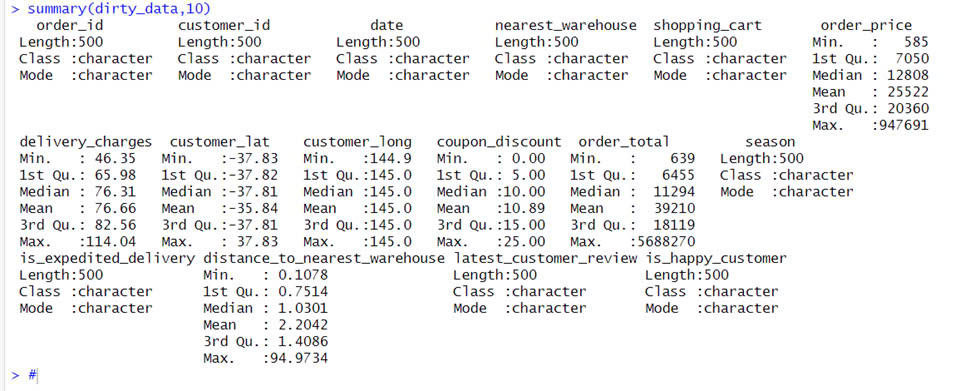
\includegraphics[width=0.9\linewidth]{graphics/bang1.jpg}
    \caption{Số liệu tổng quát}
    
\end{figure}
Sau đó ta chọn lọc những biến có thể phân tích như nearest\_warehouse, order\_price, delivery\_charges, customer\_lat, customer\_long, coupon\_discount, order\_total, season, is\_expedited\_delivery, distance\_to-\\\_nearest\_warehouse, is\_happy\_customer. Và ta có bảng dữ liệu từ lệnh \texttt{head()}.
\begin{figure}[H]
    \centering
    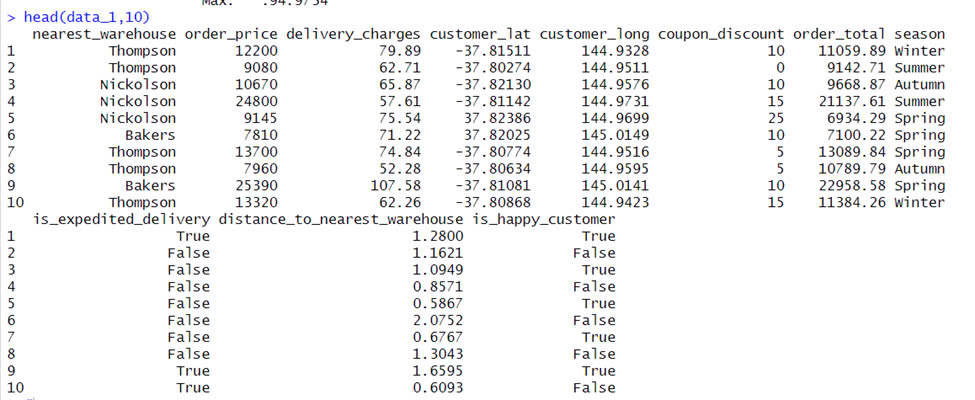
\includegraphics[width=0.9\linewidth]{graphics/bang2.jpg}
    \caption{Số liệu chọn lọc}
   
\end{figure}
            
Từ nội dung của bảng dữ liệu trên, ta tách ra thành:\\
•  Biến liên tục gồm: order\_price, delivery\_charges, customer\_lat, customer\_long, coupon\_discount, order\_total, distance\_to\_nearest\_warehouse.
 \begin{figure}[H]
    \centering
    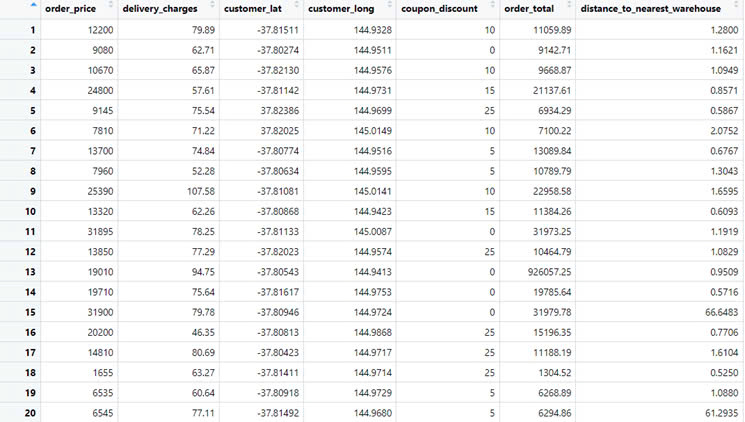
\includegraphics[width=0.9\linewidth]{graphics/bang3.jpg}
    \caption{Các biến liên tục}
   
\end{figure}
•  Biến định lượng gồm: nearest\_warehouse, season, is\_expedited\_delivery, is\_happy\_customer. Và biến định lượng được biểu diễn dưới dạng factor như sau.
\begin{figure}[H]
    \centering
    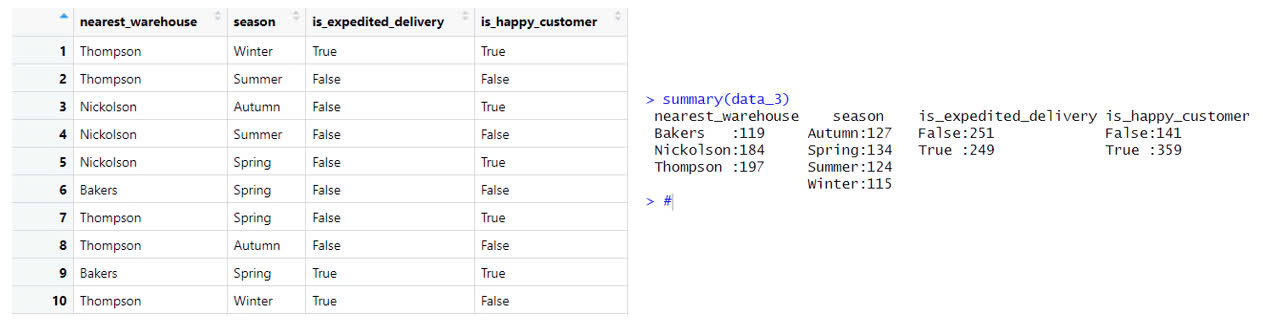
\includegraphics[width=0.9\linewidth]{graphics/bang6.jpg}
    \caption{Các biến định lượng và giá trị được biểu diễn dưới dạng factor}
   
\end{figure}
\subsection{Phân tích biến liên tục bằng biểu đồ.}
\subsubsection{Đồ thị Histogram}
•	Vì nhóm làm phân tích các ảnh hướng đến chi phí đơn hàng nên sẽ không có customer\_lat và customer\_long. Dưới đây là một số hình ảnh của các biến order\_price, delivery\_charges, coupon\_discount, order\_total, distance\_to\_nearest\_warehouse. Khi biểu diễn bằng đồ thị Histogram

\begin{figure}[H]
    \centering
    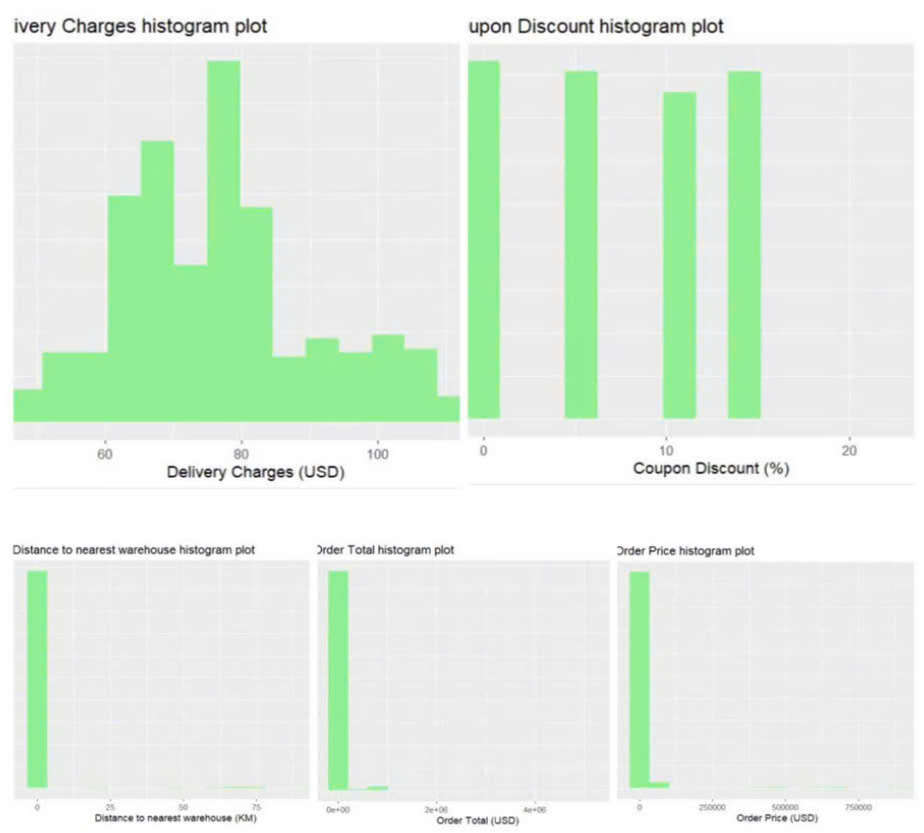
\includegraphics[width=0.7\linewidth]{graphics/bang7.jpg}
    \caption{Đồ thị Histogram của các biến liên tục}
  
\end{figure}
* Nhận xét: Ta nhận thấy rằng, từ kết quả đồ thị histogram cho thấy biến order\_total, order\_price, distance\_to\_nearest\_warehouse có phân phối lệch phải, với một cột cao ở phía bên trái. Điều này cho thấy hầu hết khách hàng chỉ chi tiêu ở mức thấp hơn, trong khi một số ít có tổng giá trị đơn hàng cao, tạo ra các điểm ngoại lệ. Phân phối lệch phải thường cho thấy  rằng có một số khách hang chi tiêu rất cao, điều này có thể ảnh hưởng đến quy mô hình hồi quy. Sau khi kiểm tra tỉ lệ khuyết nhỏ của các ngoại lai .Để xử lí tình trạng phân phối lệch phải này.\\
 -->Ta áp dụng xóa bỏ các ngoại lai  của order\_total, order\_price, distance\_to\_nearest\_warehouse.\\
 Dưới đây là hình ảnh sau khi xóa ngoại lai.
 \begin{figure}[H]
    \centering
    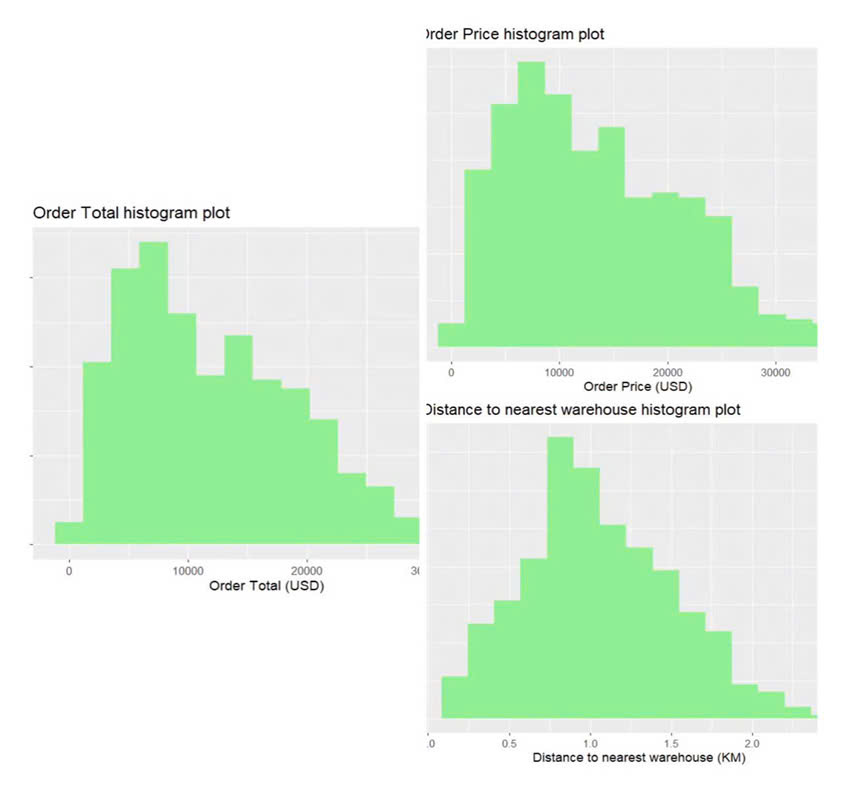
\includegraphics[width=0.7\linewidth]{graphics/bang8.jpg}
    \caption{Đồ thị Histogram của các biến liên tục đã xóa ngoại lai}
    
\end{figure}
\subsubsection{Đồ thị phân tần}
Ta so sánh  lần lượt từng order\_price, delivery\_charges, coupon\_discount, distance\_to\_nearest\_warehouse với order\_total.
\begin{figure}[H]
    \centering
    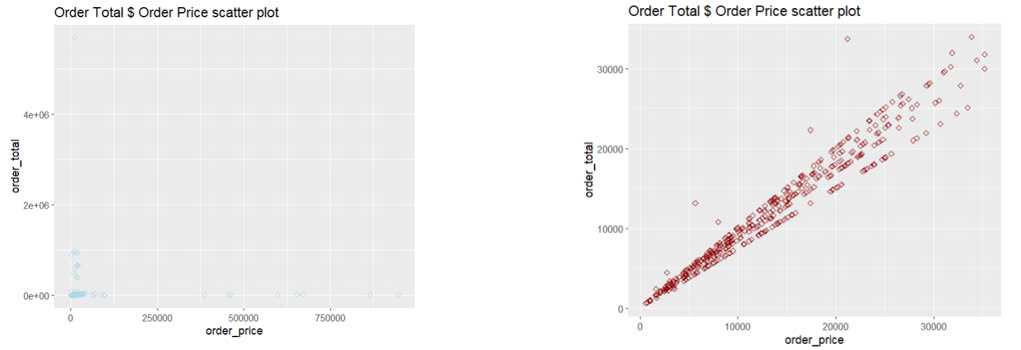
\includegraphics[width=0.8\linewidth]{graphics/bang9.jpg}
    \caption{Hình chưa xóa ngoại lai và đã xóa của order\_price}
 
\end{figure}
\begin{figure}[H]
    \centering
    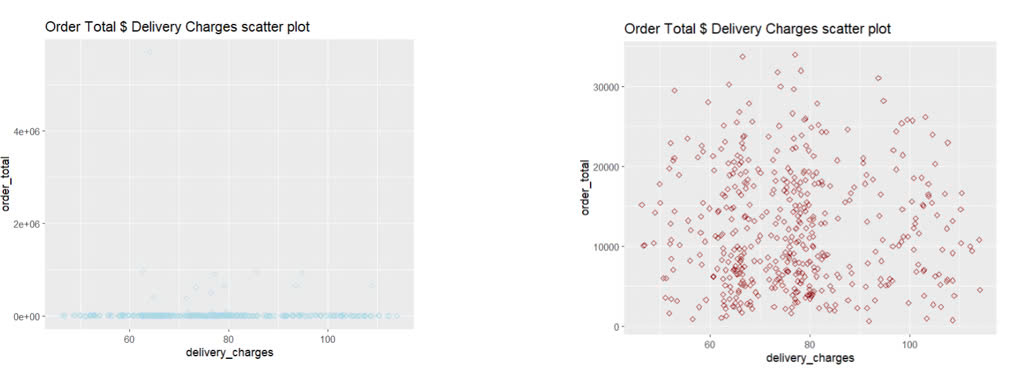
\includegraphics[width=0.8\linewidth]{graphics/bang10.jpg}
    \caption{Hình chưa xóa ngoại lai và đã xóa của delivery\_charges}
    
\end{figure}
\begin{figure}[H]
    \centering
    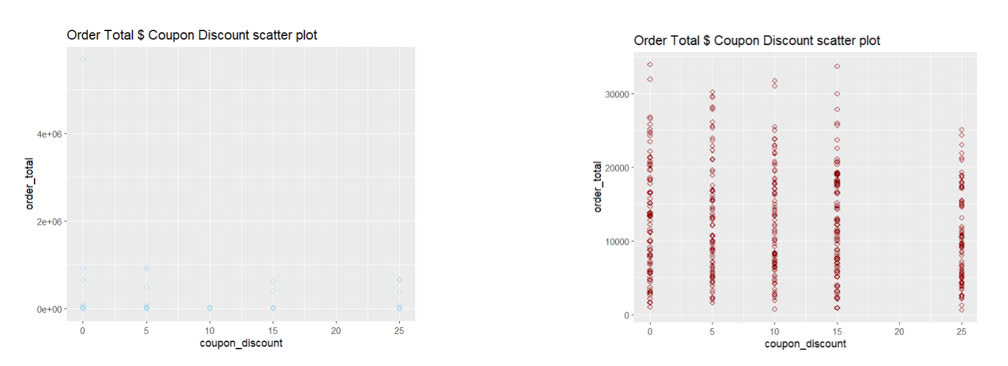
\includegraphics[width=0.8\linewidth]{graphics/bang11.jpg}
    \caption{Hình chưa xóa ngoại lai và đã xóa của coupon\_discount}
    
\end{figure}
\begin{figure}[H]
    \centering
    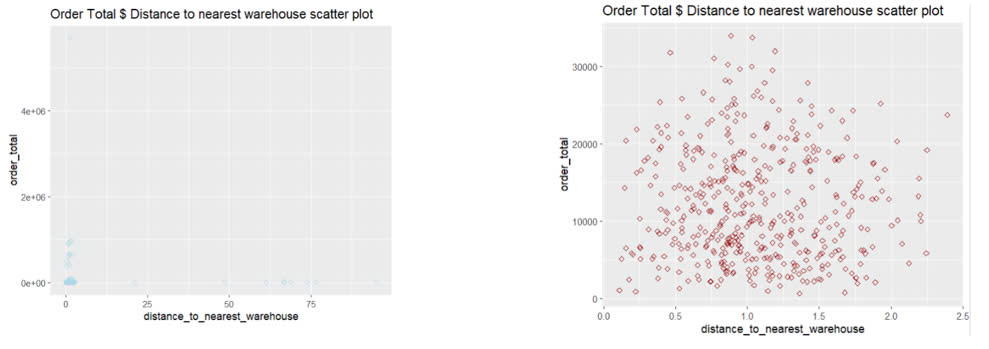
\includegraphics[width=0.8\linewidth]{graphics/bang12.jpg}
    \caption{Hình chưa xóa ngoại lai và đã xóa của distance\_to\_nearest\_warehouse}
 
\end{figure}
Với những hình ảnh có những chấm màu xanh là chưa xóa ngoại lai, còn những hình có chấm màu đỏ là đã xóa ngoại lai. \\
*Nhận xét: \\
•	Hai biến order\_price và coupon\_discount là 2 biến có ảnh hưởng tới order\_total hay còn gọi là có quan hệ tuyến tính.\\
•	Hai biến delivery\_charges và distance\_to\_nearest\_warehouse không có ảnh hưởng tới order\_total hay không có quan hệ tuyến tính.
\subsubsection{Phân tích biến định lượng bằng biểu đồ boxplot}
Ta phân tích biến order\_total theo các biến nearest\_warehouse, season, is\_expedited\_delivery, is\_happy\_customer.
\begin{figure}[H]
    \centering
    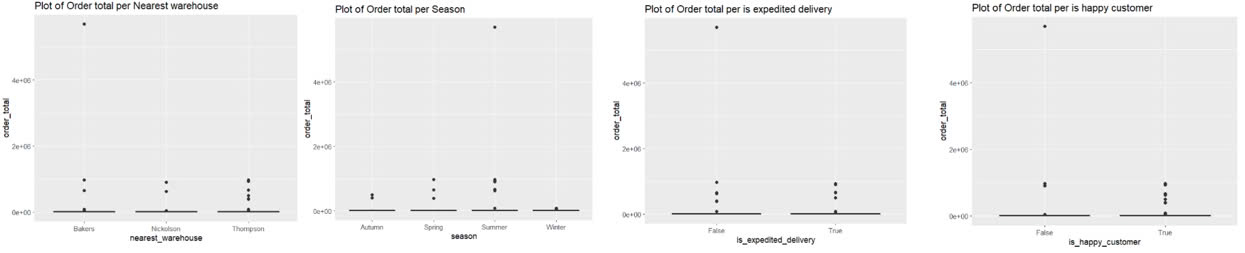
\includegraphics[width=1\linewidth]{graphics/bang13.jpg}
    \caption{Biểu đồ boxplot chưa xóa ngoại lai của các biến định lượng}
    
\end{figure}
\begin{figure}[H]
    \centering
    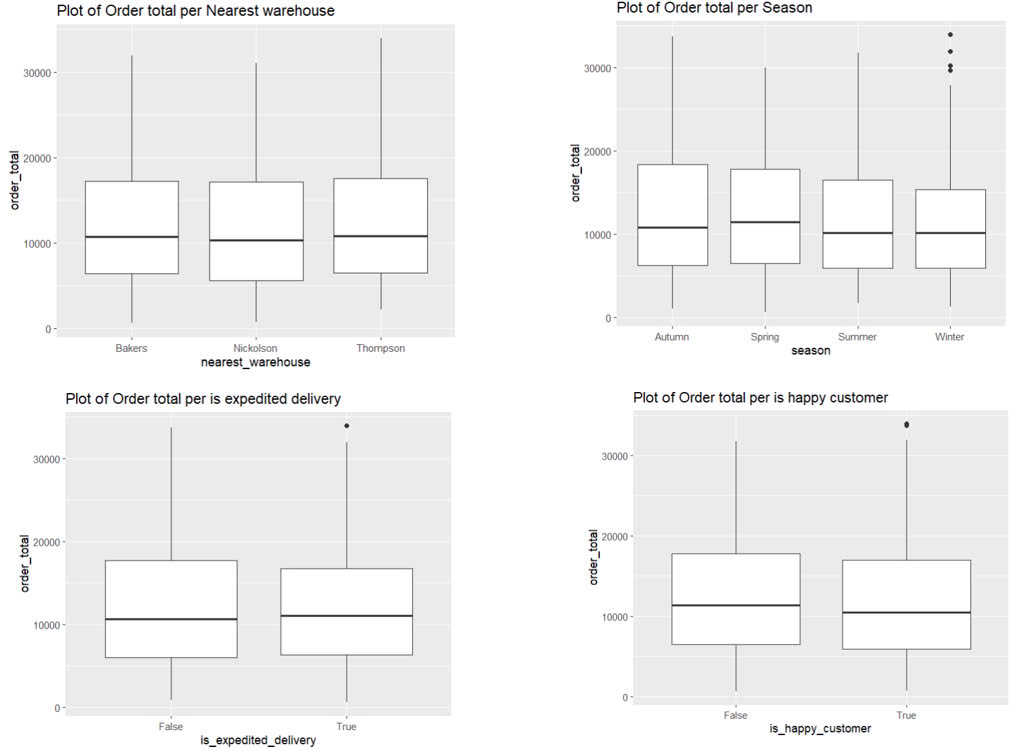
\includegraphics[width=1\linewidth]{graphics/bang14.jpg}
    \caption{Biểu đồ boxplot đã xóa ngoại lai của các biến định lượng}
    
\end{figure}
*Nhận xét: lần lượt cho  nearest\_warehouse, season, is\_expedited\_delivery, is\_happy\_customer.\\
•	Cả ba kho hàng (Bakers, Nickolson, Thompson) đều có phân bố tổng đơn hàng tương tự nhau, với các giá trị trung vị (median) gần như ngang bằng.\\
•	Phân bố giá trị order\_total khá đồng đều qua các mùa, tuy nhiên mùa Đông có một vài đơn hàng nổi bật với giá trị rất lớn.\\
•	Hình thức giao hàng nhanh dường như không có ảnh hưởng rõ rệt đến tổng giá trị đơn hàng trong phần lớn các trường hợp.\\
•	Trạng thái hài lòng của khách hàng không tạo ra sự khác biệt lớn trong tổng giá trị đơn hàng, nhưng nhóm khách hàng hài lòng có xu hướng chi tiêu nhiều hơn một chút và có thể thực hiện các đơn hàng có giá trị rất lớn (outliers).
\subsection{Bảng tương quan giữa các biến}
Bảng đánh giá tương quan trong đồ thị trên được sử dụng để hiểu rõ mối quan hệ giữa các biến số trong tập dữ liệu.
\begin{figure}[H]
    \centering
    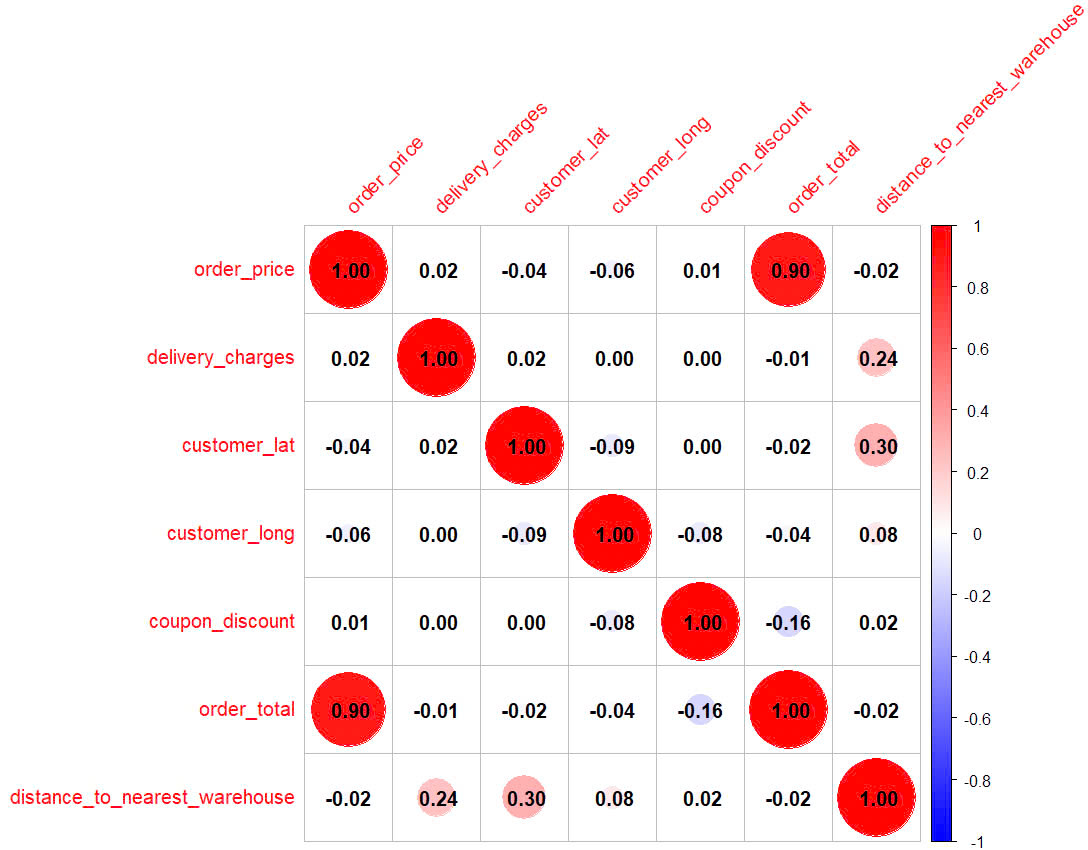
\includegraphics[width=0.8\linewidth]{graphics/tq.jpg}
    \caption{Biểu đồ tương quan của các biến}
    
\end{figure}

*Nhận Xét:

- order\_price và order\_total (tương quan: +0.90):
Đây là mối tương quan dương mạnh. Khi giá trị của order\_price tăng, order\_total cũng tăng mạnh theo và ngược lại. Điều này dễ hiểu vì order\_price là một thành phần chính của order\_total.

- distance\_to\_nearest\_warehouse và customer\_lat (+0.30):
Có mối tương quan dương trung bình giữa khoảng cách đến kho hàng và vĩ độ của khách hàng. Điều này có thể ngụ ý rằng vị trí kho hàng có xu hướng gần các khu vực cụ thể về mặt địa lý.

- distance\_to\_nearest\_warehouse và delivery\_charges (+0.24):
Mối tương quan dương nhẹ cho thấy khoảng cách đến kho hàng có tác động nhỏ đến chi phí giao hàng. Khoảng cách lớn hơn thường đi kèm với phí giao hàng cao hơn.

- order\_price và delivery\_charges (+0.02):
Hầu như không có mối liên hệ giữa giá trị đơn hàng và phí giao hàng. Điều này có thể chỉ ra rằng phí giao hàng không phụ thuộc vào giá trị đơn hàng mà dựa trên các yếu tố khác như khoảng cách hoặc chính sách giao hàng.

- coupon\_discount với hầu hết các biến khác (gần 0):
Mức giảm giá từ phiếu coupon không có mối liên hệ đáng kể với bất kỳ biến nào trong tập dữ liệu, kể cả order\_total. Điều này có thể ngụ ý rằng chiến lược giảm giá không ảnh hưởng rõ ràng đến hành vi mua sắm của khách hàng.
\section{Thống kê suy diễn}
\subsection{Phân tích phương sai một nhân tố (One-way ANOVA)} \label{anova1}
\subsubsection{Mục đích}
Đánh giá xem biến nhân tố X có ảnh hưởng đến biến phụ thuộc Y hay không? Trong đề tài này chúng ta sẽ kiểm định xem, việc các mùa (season) cũng như hình thức giao hàng nhanh (is\_expedited\_delivery) sẽ ảnh hưởng như thế nào đến phí giao hàng (delivery\_charges) bằng phương pháp phân tích phương sai ANOVA một nhân tố.
\subsubsection{Tiến hành phân tích}
%yêu mùa ảnh hưởng tới phí giao hàng
Đầu tiên chúng ta sẽ kiểm định xem, việc các mùa (season) ảnh hưởng như thế nào đến phí giao hàng (delivery\_charges) bằng phương pháp phân tích phương sai ANOVA một nhân tố. .Hình \ref{fig:5.1} thể hiện kết quả phân tích phương sai ANOVA một nhân tố cho mẫu thống kê bằng câu lệnh chính là anova1 <- aov(delivery\_charges ~ season, data=loi1) Trong RStudio (xem code từ dòng 381 đến 389 trong file: codeR\_nhom10\_lopTN01.r).
\begin{figure}[!htbp]
    \centering
    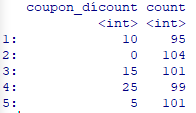
\includegraphics[width=0.6\linewidth]{graphics/5.3.1.png}
    \caption{Phân tích phương sai ANOVA xét sự ảnh hưởng của mùa (season) đến phí giao hàng (delivery\_charges)}
    \label{fig:5.1}
\end{figure}
Quan sát kết quả trên hình \ref{fig:5.1}, giá trị p-value (tức Pr(>F)) là rất rất nhỏ hơn ngưỡng ý nghĩa phổ biến (0.05). Do đó, cho thấy sự khác biệt rất có ý nghĩa thống kê, có đủ bằng chứng thống kê rất mạnh để kết luận rằng, các mùa (season) có ảnh hưởng rất mạnh đến phí giao hàng (delivery\_charges).

Để xác định trung bình của nhóm nào là khác biệt, ta sử dụng phương pháp so sánh bội (Multiple comparison method). Một phương pháp so sánh bội đơn giản và có ý nghĩa độ lệch nhỏ nhất (Least significant difference - LSD) của Fisher. Hình \ref{fig:5.2} thể hiện kết quả của phương pháp so sánh bội Least significant difference - LSD bằng câu lệnh chính là lsd1<- LSD.test(anova1, "season", console=TRUE) trong thư viện library(agricolae) Trong RStudio (xem code dòng 392 trong file: codeR\_nhom10\_lopTN01.r)
\begin{figure}[!htbp]
    \centering
    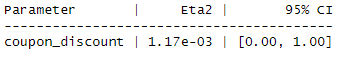
\includegraphics[width=0.6\linewidth]{graphics/5.3.3.png}
    \caption{So sánh bội sau anova của mùa}
    \label{fig:5.2}
\end{figure}
Từ kết quả ở hình trên ta thấy được trung bình, độ lệch chuẩn (Std), số mẫu (r), độ lệch chuẩn trung bình (SE), cận trên của khoản tin cậy (LUL), cận dưới của khoản tin cậy (UCL) đồng thời phân nhóm ý nghĩa. Thông qua phân nhóm ý nghĩa cho thấy mùa thu(Autumn) và mùa đông (Winter) không khác biệt nhau lắm còn mùa hè(Summer) cao hơn và mùa xuân(Spring) là phí giao hàng cao nhất, khác biệt đáng kể nhất so với các mùa còn lại.
%yêu cầu giao hàng nhanh ảnh hưởng tới phí giao hàng

Tiếp theo chúng ta sẽ tiếp tục kiểm định thêm một yếu tố nữa là việc khách hàng yêu cầu giao hàng nhanh (is\_expedited\_delivery) sẽ ảnh hưởng như thế nào đến phí giao hàng (delivery\_charges) bằng phương pháp phân tích phương sai ANOVA một nhân tố. Hình \ref{fig:5.2} thể hiện kết quả phân tích phương sai ANOVA một nhân tố cho mẫu thống kê bằng câu lệnh chính là anova11 <- aov(delivery\_charges ~ is\_expedited\_delivery, data=loi2) Trong RStudio (xem code từ dòng 393 đến 400 trong file: codeR\_nhom10\_lopTN01.r).
\begin{figure}[!htbp]
    \centering
    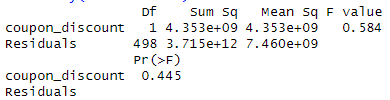
\includegraphics[width=0.7\linewidth]{graphics/5.3.2.png}
    \caption{Phân tích phương sai ANOVA xét sự ảnh hưởng của việc khách hàng yêu cầu giao hàng nhanh (is\_expedited\_delivery) đến phí giao hàng(delivery\_charges)}
    \label{fig:5.3}
\end{figure}
Quan sát kết quả trên hình \ref{fig:5.3}, giá trị p-value (tức Pr(>F)) là rất rất nhỏ hơn ngưỡng ý nghĩa phổ biến (0.05). Do đó, cho thấy sự khác biệt rất có ý nghĩa thống kê, có đủ bằng chứng thống kê rất mạnh để kết luận rằng, việc khách hàng yêu cầu giao hàng nhanh (is\_expedited\_delivery) có ảnh hưởng rất mạnh đến phí giao hàng (delivery\_charges).

Để xác định trung bình của nhóm nào là khác biệt, ta sử dụng phương pháp so sánh bội (Multiple comparison method). Một phương pháp so sánh bội đơn giản và có ý nghĩa độ lệch nhỏ nhất (Least significant difference - LSD) của Fisher. Hình \ref{fig:5.4} thể hiện kết quả của phương pháp so sánh bội Least significant difference - LSD bằng câu lệnh chính là lsd2<- LSD.test(anova11, "is\_expedited\_delivery", console=TRUE)
trong thư viện library(agricolae) Trong RStudio (xem code dòng 405 trong file: codeR\_nhom10\_lopTN01.r)
\begin{figure}[!htbp]
    \centering
    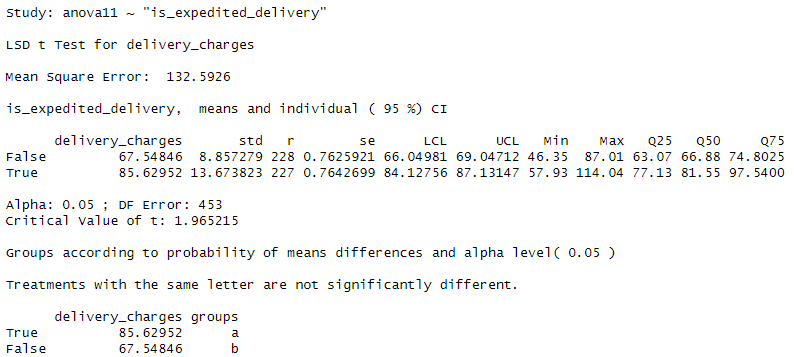
\includegraphics[width=0.6\linewidth]{graphics/5.3.4.png}
    \caption{So sánh bội sau anova của yêu cầu giao hàng nhanh}
    \label{fig:5.4}
\end{figure}
Từ kết quả ở hình trên ta thấy được trung bình, độ lệch chuẩn (Std), số mẫu (r), độ lệch chuẩn trung bình (SE), cận trên của khoản tin cậy (LUL), cận dưới của khoản tin cậy (UCL) đồng thời phân nhóm ý nghĩa. Thông qua phân nhóm ý nghĩa cho thấy việc yêu cầu giao hàng nhanh và không yêu cầu giao hàng nhanh có khác biệt đáng kể.

\subsubsection{Kết luận}
Phân tích ANOVA 1 nhân tố cho thấy season, is\_expedited\_delivery, một cách riêng biệt, có ảnh hưởng đáng kể đến delivery\_charges.

\subsection{Phân tích phương sai hai nhân tố (Two-factor ANOVA)}
\subsubsection{Mục đích}
Trong phần nghiên cứu này, chúng tôi sẽ sử dụng ANOVA 2 yếu tố không lặp để phân tích xem liệu \textbf{Được giao hàng nhanh (is\_expedited\_delivery)} và \textbf{Mùa (season)} có ảnh hưởng đến \textbf{Phí giao hàng (delivery\_charges)} hay không?

Giả thiết thống kê được thực hiện với mức ý nghĩa $\alpha = 0.05$.


\begin{itemize}
    
    \item Kiểm định yếu tố A (is\_expedited\_delivery)
    \begin{itemize}
        \item Đánh giá xem biến nhân tố A có ảnh hưởng đến biến phụ thuộc hay không?
        
        \[
            H_{0A}: \tau_{1} = \tau_{2} = \tau_{3} = \dots = \tau_{a} = 0
            \]
            \[
            H_{1A}: \tau_{i} \neq  0 \text{ với ít nhất một i }
            \]
    \end{itemize}
    
    \item Kiểm định yếu tố B (season)
    \begin{itemize}
        \item Đánh giá xem biến nhân tố B có ảnh hưởng đến biến phụ thuộc hay không?
        
        \[
            H_{0B}: \beta_{1} = \beta_{2} = \beta_{3} = \dots = \beta_{b} = 0
            \]
            \[
            H_{1B}: \beta_{j} \neq  0 \text{ với ít nhất một j }
            \]
    \end{itemize}
    \item Đối với tương tác giữa A và B  
    \begin{itemize}
        \item Đánh giá xem các biến nhân tố A và B có tương tác với nhau hay không?
        
        \[
            H_{0AB}: \tau\beta_{11} = \tau\beta_{12}  = \dots = \tau\beta_{AB} = 0 
            \]
            \[
            H_{1AB}: \tau\beta_{ij} \neq  0 \text{ với ít nhất một cặp (i,j) }
            \]
    \end{itemize}
\end{itemize}
\subsubsection{Kiểm tra điều kiện cho dữ liệu}
Trước khi tiến hành phân tích ANOVA 2 chiều, ta cần kiểm tra các điều kiện cần thiết cho dữ liệu:


 Đầu tiên ta kiểm tra xem dữ liệu của \textbf{Biến phụ thuộc:} \textbf{delivery\_charges} ở mỗi nhóm do tổ hợp các mức của hai nhân tố tạo ra có tuân theo phân phối chuẩn không.
 \begin{figure}[!htbp]
    \centering
    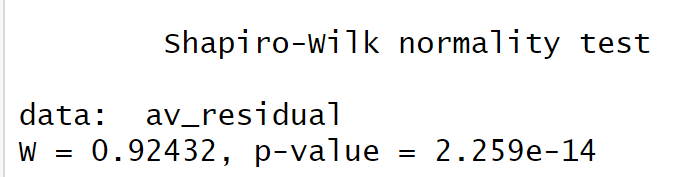
\includegraphics[width=0.7\linewidth]{graphics/5.4.1 (2).png}
    \caption{Kết quả kiểm tra phân phối chuẩn}
\end{figure}
\FloatBarrier

Có thể thấy p\_value < 0. 05 dữ liệu không tuân theo phân phối chuẩn.
Tuy dữ liệu không tuân theo quy luật phân phối chuẩn nhưng mẫu đủ lớn, ta vẫn có thể sử dụng mô hình anova mà không cần lo ngại quá nhiều về vấn đề phân phối chuẩn của dữ liệu. Điều này dựa trên lý thuyết \textbf{Lý thuyết Giới hạn Trung tâm (Central Limit Theorem - CLT)}. 


   Tiếp theo, ta kiểm tra xem các nhóm được phân tích ở trên có phương sai đồng nhất hay không 

   \begin{figure}[!htbp]
    \centering
    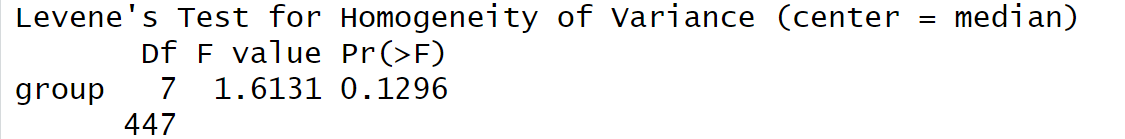
\includegraphics[width=0.7\linewidth]{graphics/5.4.2.png}
    \caption{Kết quả kiểm tra phương sai đồng nhất}
\end{figure}

Có thể thấy giá trị p > 0.05 nên các nhóm có phương sai đồng nhất . 
Sau khi đã thỏa mãn các điểu kiện kiểm tra dữ liệu ta tiến hành phân tích ANOVA 2 chiều.

\subsubsection{Tiến hành phân tích}


        Dựa vào bảng dữ liệu ta có thể thấy sự tương tác giữa 2 nhân tố is\_expedited\_delivery và season

        \begin{figure}[!htbp]
            \centering
            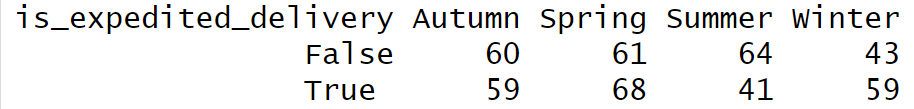
\includegraphics[width=1\linewidth]{graphics/5.4.3.png}
            \caption{bảng dữ liệu}
        \end{figure}
        Kết quả nhận được: 

        \begin{figure}[!htbp]
            \centering
            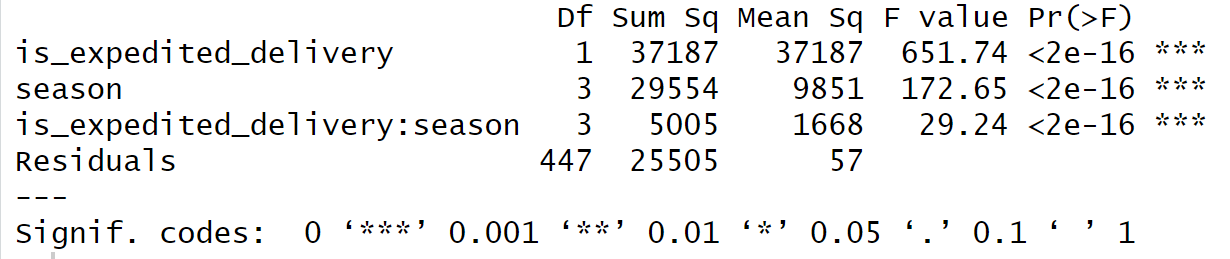
\includegraphics[width=1\linewidth]{graphics/5.4.4.png}
            \caption{Phân tích anova 2 yếu tố}
        \end{figure}

        Chúng tôi tiến hành phân tích ANOVA 2 chiều trong phần phần mềm R. 
        Kết quả và nhận xét: 
        Kết quả phân tích ANOVA hai yếu tố được trình bày trong hình 5.4. Kết quả cho thấy rằng cả ba yếu tố \textbf{season}, \textbf{is\_expedited\_delivery}, và sự tương tác giữa chúng đều có ảnh hưởng đáng kể đến \textbf{delivery\_charges} với mức ý nghĩa $\alpha = 0.05$. Dưới đây là các nhận xét chi tiết:

        \begin{itemize}
    \item \textbf{Tương tác giữa season và is\_expedited\_delivery}:
    \begin{itemize}
        \item Với \textbf{Df = 3}, có 3 mức độ tương tác giữa hai yếu tố \textbf{season} và \textbf{is\_expedited\_delivery}.
        \item Giá trị \textbf{F = 29.24} và \textbf{Pr(>F) = 2e-16***} cho thấy rằng có sự tương tác có ý nghĩa thống kê giữa hai yếu tố này và ảnh hưởng đến \textbf{delivery\_charges}. Do đó, ta bác bỏ giả thuyết không \(H_0\) cho sự tương tác này.
    \end{itemize}

    \end{itemize}

 Từ những kết quả trên, chúng tôi kết luận rằng cả yếu tố \textbf{season}, \textbf{is\_expedited\_delivery}, và sự tương tác giữa chúng đều có ảnh hưởng quan trọng và có ý nghĩa thống kê đối với \textbf{delivery\_charges}. Điều này cho thấy rằng các yếu tố này cần được cân nhắc kỹ lưỡng khi định giá sản phẩm.
               
        
\subsubsection{Kết luận}
Phân tích ANOVA 2 chiều cho thấy \textbf{season}, \textbf{is\_expedited\_delivery}, và sự tương tác giữa chúng đều có ảnh hưởng đáng kể đến \textbf{delivery\_charges}. Mặc dù có một số hạn chế về phân phối chuẩn , kết quả này vẫn cung cấp cơ sở tin cậy để đánh giá và điều chỉnh chiến lược giá sản phẩm.
\subsection{Hồi quy tuyến tính đa bội}
\subsubsection{Mục đích}

Mục đích của mô hình hồi quy tuyến tính này là dự đoán giá trị tổng đơn hàng dựa trên các yêu tố giải thích khác nhau như giá trị đơn hàng, phí vận chuyển,..

\subsubsection{Kiểm tra dữ liệu có tuân theo phân phối chuẩn hay không} 

Ta cần kiểm tra xem các dữ liệu của ta có tuân theo quy luật phận phối chuẩn hay không bằng cách cho mức ý nghĩa là 5\%, ta dùng lệnh \textbf{shapiro.test()} để kiểm tra p-value. Nếu giá trị p-value > 0.05, thì cột dữ liệu đó tuân theo phân phối chuẩn và ngược lại.Thực hiện trên Rstudio ta thu được kết quả:


\begin{figure}[!htp]
  \centering
  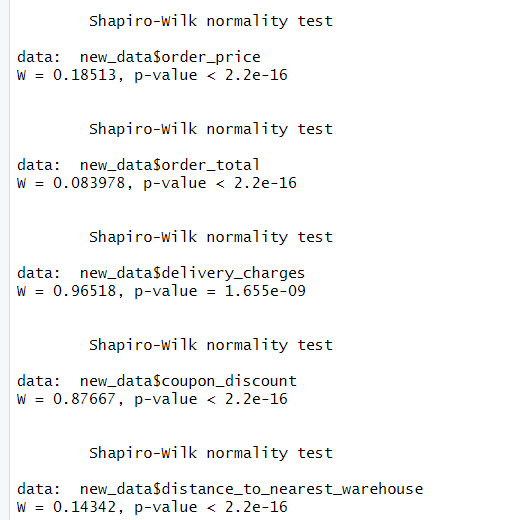
\includegraphics[width=0.7\linewidth]{graphics/5.5.0.png}
  \caption{kết quả kiểm  tra phân phối chuẩn của các biến }
\end{figure}

5 cột dữ liệu đều có p-value < 0.05, điều đó cho ta thấy cả 5 cột không tuân theo quy luật phân phối chuẩn.

Tuy dữ liệu không tuân theo quy luật phân phối chuẩn nhưng mẫu đủ lớn, ta vẫn có thể sử dụng hồi quy tuyến tính mà không cần lo ngại quá nhiều về vấn đề phân phối chuẩn của dữ liệu. Điều này dựa trên lý thuyết \textbf{Lý thuyết Giới hạn Trung tâm (Central Limit Theorem - CLT)}. 

Lý thuyết Giới hạn Trung tâm là một khái niệm quan trọng trong thống kê vì nó cho phép chúng ta làm việc với các mẫu ngẫu nhiên mà không cần phải lo lắng về phân phối gốc của dữ liệu. Nó đảm bảo rằng, khi kích thước mẫu đủ lớn, các phân tích thống kê có thể sử dụng phân phối chuẩn để thực hiện các ước lượng và kiểm định giả thuyết, ngay cả khi dữ liệu gốc không tuân theo phân phối chuẩn.
\subsubsection{Xây dựng mô hình hồi quy tuyến tính}
Trước tiên ta kiểm tra sự phụ thuộc của biến delivery\_charges vào hai biến độc lập is\_expedited\_delivery và distance\_to\_nearest\_warehouse. Ta sử dụng lệnh lm().

Kết quả phân tích trên Rstudio:
\begin{figure}[!htp]
  \centering
  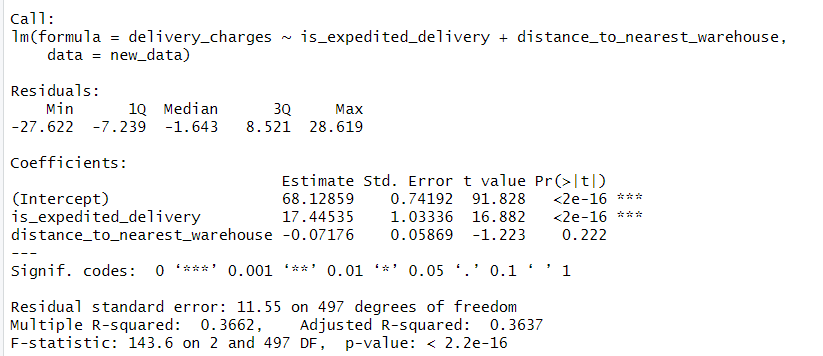
\includegraphics[width=0.7\linewidth]{graphics/5.5.1.png}
  \caption{Kết quả hồi quy tuyến tính giữa 2 biến delivery\_charges và is\_expedited\_delivery  }
\end{figure}


Với mức ý nghĩa 5\%, ta phân tích phần Coefficients (hệ số) như sau:

Định nghĩa biến $x_1$: is\_expedited\_delivery,$x_2$:distance\_to\_nearest\_warehouse, y:delivery\_charges

Cho biết hệ số của biến độc lập trong phương trình: $\beta_0= 68.12859, \beta_1= 17.44535,\\ \beta_2= -0.07176 $
 
Ta có phương trình hồi quy tuyến tính đơn giản: $y= 68.12859 + 17.44535x_1 - 0.07176x_2$

 Dựa vào bảng số liệu trên ta có:\\
 \begin{itemize}
 \item\textbf{Pr(>|t|)}: Chỉ có giá trị p-value của biến distance\_to\_nearest\_warehouse lớn hơn 0.05(0.222>0.05), cho thấy biến distance\_to\_nearest\_warehouse không có ý nghĩa thống kê trong mô hình này. Có thể xem như hai biến delivery\_charges và distance\_to\_nearest\_warehouse độc lập với nhau.
\item\textbf{Multiple R-squared}: 0.3662, cho thấy mô hình giải thích được 36.62\% biến động của delivery\_charges.
 \end{itemize}

 Mô hình hồi quy này chỉ ra rằng việc giao hàng nhanh \textbf{(is\_expedited\_delivery)} có ảnh hưởng đáng kể và có ý nghĩa thống kê đến chi phí giao hàng \textbf{(delivery\_charges)}. Mặc dù mô hình giải thích được \textbf{36.62\%} biến động của chi phí giao hàng, điều này cho thấy vẫn còn nhiều yếu tố khác cần được xem xét để giải thích toàn bộ biến động của chi phí giao hàng.

Trên thực tế tổng giá trị đơn hàng phụ thuộc vào tổng giá trị mặt hàng, chi phí vận chuyển, mã giảm giá, khoảng cách đến kho hàng gần nhất,....Vậy nên ta chọn biến \textbf{order\_total} làm biến phụ thuộc vào các biến độc lập \textbf{order\_price, delivery\_charges},\textbf{coupon\_discount} và \textbf{distance\_to\_nearest\_warehouse}.

Ta xét khi có các biến ngoại lai. Hồi quy tuyến tính mô hình trên ta có được:
\begin{figure}[!htp]
  \centering
  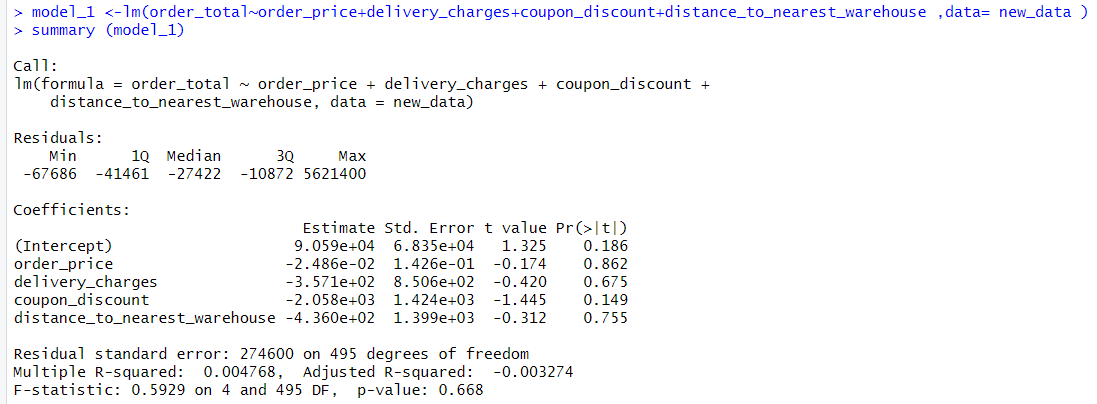
\includegraphics[width=0.7\linewidth]{graphics/5.5.2.png}
  \caption{Kết quả hồi quy tuyến tính mô hình 1 }
\end{figure}

Dựa trên kết qủa từ hàm \textbf{summary(model\_1)} ta rút ra nhận xét sau:
\begin{itemize}
\item \textbf{(Intercept)}: Khi tất cả các biến độc lập bằng 0, giá trị trung bình của order\_total là 90590. Tuy nhiên, giá trị p-value là 0.186, không có ý nghĩa thống kê.
\item \textbf{order\_price}: Hệ số ước lượng là -0.02486, và p-value là 0.862, không có ý nghĩa thống kê.
\item \textbf{delivery\_charges}: Hệ số ước lượng là -357.1, và p-value là 0.675, không có ý nghĩa thống kê.
\item \textbf{coupon\_discount}: Hệ số ước lượng là -2058.0, và p-value là 0.149, không có ý nghĩa thống kê.
\item \textbf{distance\_to\_nearest\_warehouse}: Hệ số ước lượng là -436.0, và p-value là 0.755, không có ý nghĩa thống kê.
\item\textbf{Multiple R-squared}: 0.004768, chỉ ra rằng mô hình chỉ giải thích được 0.4768\% biến động của order\_total.
\item\textbf{F-statistic}: 0.5929, với p-value là 0.668, cho thấy mô hình tổng thể không có ý nghĩa thống kê
\end{itemize}
Mô hình hồi quy model\_1 không phù hợp tốt với dữ liệu của bạn bởi vì:
\begin{itemize}
\item Các biến độc lập đều không có ý nghĩa thống kê ($p-value > 0.05$).
\item Chỉ số \textbf{R-squared} rất thấp, cho thấy mô hình không giải thích được biến động của order\_total.
\item\textbf{F-statistic} không có ý nghĩa thống kê, gợi ý rằng mô hình tổng thể không phù hợp.
\end{itemize}

Tiếp theo ta xét tiếp khi bỏ các giá trị ngoại lai

Hồi quy trên Rstudio ta có được:
\begin{figure}[!htp]
  \centering
  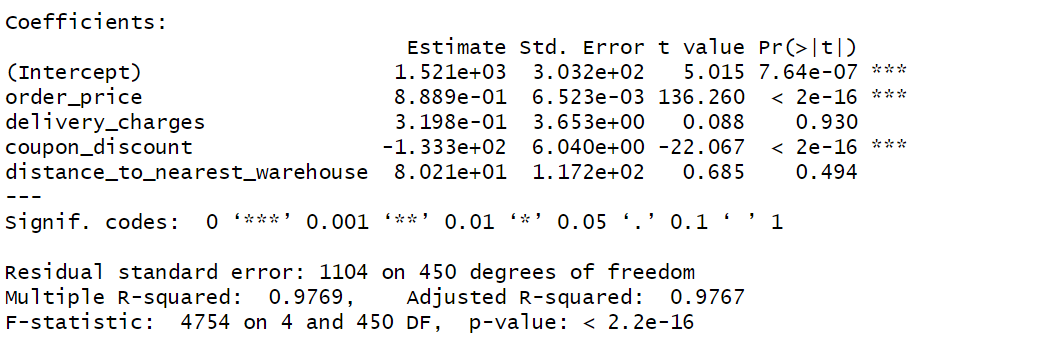
\includegraphics[width=0.7\linewidth]{graphics/5.5.3.png}
  \caption{Kết quả hồi quy tuyến tính mô hình 2 }
\end{figure} 

Dựa trên kết quả từ hàm \textbf{summary(model\_2)}, ta có thể rút ra các nhận xét:

Với mức ý nghĩa 5\%, ta phân tích phần Coeficients(hệ số) như sau:

Định nghĩa các biến:  y: order\_total, $x_1$: order\_price, $x_2$: delivery\_charges, $x_3$: coupon\_discount, $x_4$: distance\_to\_nearest\_warehouse.

Cho các hệ số của từng biến độc lập trong phương trình : $\beta_0= 1450, \beta_1= 0.8887, \\\beta_2= 1.132, \beta_3= -133.9, \beta_4= 103.1$ Ta có phương trình hồi quy: 

 \hspace{25mm}$y= 1450 + 0.8887x_1 + 1.132x_2 - 133.9x_3 + 103.1x_4$

Ý nghĩa của hệ số hồi quy:
\begin{itemize}
\item\textbf{(Intercept)}: Khi tất cả các biến độc lập bằng 0, giá trị trung bình của order\_total là 1450.0. Giá trị p-value rất nhỏ (1.57e-05), có ý nghĩa thống kê.
\item\textbf{order\_price}: Hệ số ước lượng là 0.8887, và p-value rất nhỏ (< 2e-16), có ý nghĩa thống kê mạnh mẽ. Mỗi đơn vị tăng của order\_price dẫn đến order\_total tăng trung bình 0.8887 đơn vị, giữ nguyên các yếu tố khác.\\
\item\textbf{delivery\_charges}: Hệ số ước lượng là 1.132, và p-value là 0.776, không có ý nghĩa thống kê.
\item\textbf{coupon\_discount}: Hệ số ước lượng là -133.9, và p-value rất nhỏ (< 2e-16), có ý nghĩa thống kê mạnh mẽ. Mỗi đơn vị tăng của coupon\_discount dẫn đến order\_total giảm trung bình 133.9 đơn vị, giữ nguyên các yếu tố khác.
\item\textbf{distance\_to\_nearest\_warehouse}: Hệ số ước lượng là 103.1, và p-value là 0.399, không có ý nghĩa thống kê.
\end{itemize}

Chỉ số đo lường của mô hình:

\begin{itemize}
\item\textbf{Multiple R-squared}: 0.9765, cho thấy mô hình giải thích được 97.65\% biến động của order\_total.
\item\textbf{F-statistic}: 4534, với p-value < 2.2e-16, cho thấy mô hình tổng thể có ý nghĩa thống kê mạnh mẽ.
\end{itemize}

Từ 2 mô hình trên ta có thể thấy được rằng giá trị ngoại lai ảnh hưởng đến hồi quy tuyến tính như thế nào. Các giá trị ngoại lai có thể làm suy yếu mô hình hồi quy tuyến tính, làm giảm khả năng giải thích của mô hình và làm sai lệch các hệ số ước lượng. Sau khi xử lý ngoại lai, mô hình có sự cải thiện rõ rệt, với giá trị R-squared cao hơn và các biến có ý nghĩa thống kê tốt hơn. Việc loại bỏ các ngoại lai giúp làm sạch dữ liệu và cải thiện độ chính xác của mô hình.

Qua mô hình 2 ta thấy có hai biến là biến \textbf{order\_price} và \textbf{coupon\_discout} là phù hợp (p-value<0.05), vì thế nên ta loại bỏ hai biến còn lại ra khỏi mô hình.

Loại bỏ hai biến \textbf{delivery\_charges} và \textbf{distance\_to\_nearest\_warehouse}, giữ lại biến có ý nghĩa là \textbf{order\_price} và \textbf{coupon\_discount}.

Từ đó ta có mô hình 3 : $y= \beta_0 + \beta_1x_1 + \beta_2x_2$ với y: order\_total, $x_1$: order\_price, $x_2$: coupon\_discount.

Ta tiếp sử dụng Rstudio để phân tích mô hình 3
\begin{figure}[!htp]
  \centering
  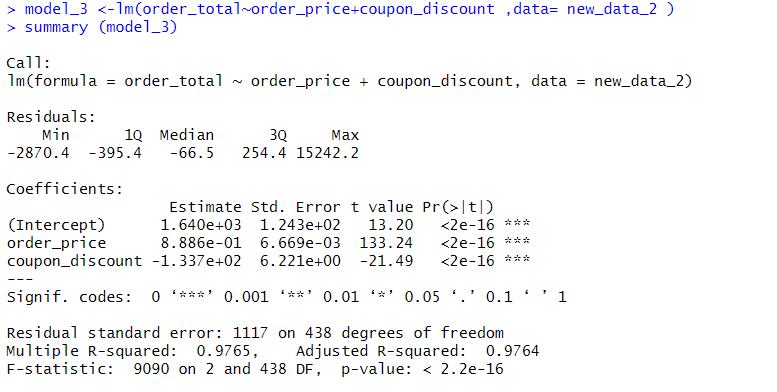
\includegraphics[width=0.7\linewidth]{graphics/5.5.4.png}
  \caption{Kết quả hồi quy tuyến tính mô hình 3 }
\end{figure}

Với mức ý nghĩa 5\% ta có phương trình: $y= 1640 + 0.8886x_1 - 133.7 x_2$

Ý nghĩa của hệ số hồi quy:
\begin{itemize}
\item\textbf{(Intercept)}: Hệ số chặn (Intercept) là 1640, có ý nghĩa thống kê mạnh (p-value < 0.001).
\item\textbf{order\_price}: Hệ số của order\_price là 0.8886, có ý nghĩa thống kê mạnh với p-value rất nhỏ (< 0.001). Điều này cho thấy mối quan hệ tích cực giữa order\_price và order\_total, tức là khi giá trị đơn hàng tăng, tổng giá trị đơn hàng cũng tăng.
\item\textbf{coupon\_discount}: Hệ số của coupon\_discount là -133.7, có ý nghĩa thống kê mạnh với p-value < 0.001. Mối quan hệ này cho thấy khi mức giảm giá (coupon) tăng lên, tổng giá trị đơn hàng giảm đi.
\end{itemize}

Chỉ số đo lường mô hình:

\begin{itemize}
\item\textbf{Multiple R-squared}: 0.9765, cho thấy mô hình giải thích được 97.65\% biến động của order\_total.
\item\textbf{F-statistic}: 9090, với p-value < 2.2e-16, cho thấy mô hình tổng thể có ý nghĩa thống kê mạnh mẽ.
\end{itemize}

Mô hình 3 có hiệu quả rất cao trong việc giải thích sự biến thiên của \textbf{order\_total}, với \textbf{R-squared} lên đến \textbf{97.65\%}. Các biến \textbf{order\_price} và \textbf{coupon\_discount} là những yếu tố quan trọng và có ảnh hưởng rõ rệt đến tổng giá trị đơn hàng. Việc loại bỏ các biến không quan trọng như \textbf{delivery\_charges} và \textbf{distance\_to\_nearest\_warehouse} giúp đơn giản hóa mô hình mà vẫn giữ được khả năng dự đoán chính xác.

\subsubsection{Kiểm định lại mô hình hồi quy tuyến tính}
Tiếp tục kiểm định, ta xác định khoảng tin cậy cho hệ số với mức ý nghĩa 5\%\ bằng lệnh \textbf{confint(model\_3)}:
\begin{figure}[!htp]
  \centering
  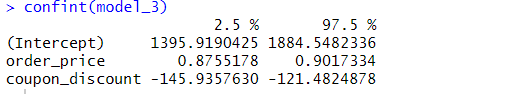
\includegraphics[width=0.7\linewidth]{graphics/5.5.5.png}
  \caption{Kiểm định khoảng tin cậy hệ số mô hình 3 }
\end{figure}

Ta thấy các hệ số $\beta_0= 1640\in(1395.91904; 1884.5482), \beta_1= 0.8886\in(.8755;0.9017),\\ \beta_2= -133.7\in(-145.9358 -121.4825)$
\paragraph{Kiểm định bằng đồ thị}

Kiểm tra giả định mô hình hồi quy tuyến tính bằng đồ thị:
\newpage

\begin{figure}[!htp]
  \centering
  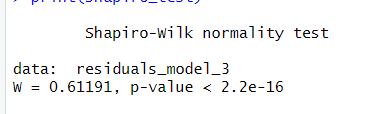
\includegraphics[width=0.7\linewidth]{graphics/5.5.6.png}
  \caption{Đồ thị kiểm định mô hình hồi quy  tuyến tính }
\end{figure}

Nhận xét dựa trên đồ thị chuẩn đoán:

\textbf{Residual vs Fitted:}
\begin{itemize}
 \item Các điểm dữ liệu không hoàn toàn phân bố ngẫu nhiên quanh đường ngang tại 0, gợi ý rằng có thể có vấn đề với tuyến tính hoặc phương sai không đồng nhất. 
\end{itemize}
 \textbf{Q-Q Residuals:}
 \begin{itemize}
\item Các điểm dữ liệu phần lớn nằm dọc theo đường chéo, nhưng có một số điểm lệch ở hai đầu Điều này gợi ý rằng phần dư có thể không hoàn toàn tuân theo phối chuẩn, nhưng sự sai lệch không quá nghiêm trọng.
 \end{itemize}
\textbf{Scale-Location:}
\begin{itemize}
\item Các điểm dữ liệu không hoàn toàn phân bố ngẫu nhiên và có xu hướng tăng lên, điều này gợi ý rằng phương sai có thể không đồng nhất.
\end{itemize}
\textbf{Residuals và Leverage:}
\begin{itemize}
\item Một số điểm có leverage cao và phần dư lớn, cho thấy một số điểm dữ liệu  có thể có ảnh hưởng mạnh đến mô hình. Những điểm này cần được kiểm tra kỹ lưỡng.
\end{itemize}
\paragraph{Kiểm định bằng thống kê}

Kiểm định bằng phương pháp so sánh với giá trị thực tế:

Ta tiến hành thay các giá trị $x_1$, $x_2$ vào phương trình(ở mô hình 3): $y= 1640 + 0.8886x_1 - 133.7 x_2$ sau đó so sánh với giá trị order\_total trong bảng. Ta sử dụng Rstudio để thực hiện thao tác trên:

\begin{figure}[!htp]
  \centering
  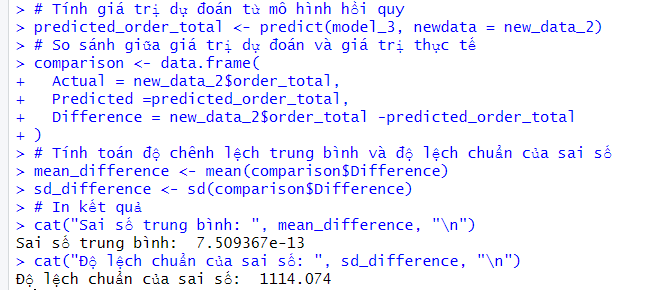
\includegraphics[width=0.5\linewidth]{graphics/5.5.7.png}
  \caption{So sánh giá trị hồi quy với giá trị thực tế }
\end{figure}

Ta sử dụng lệnh predict để tiến hành thay các giá trị vào phương trình. Sau khi tiến hành so sánh ta thu được hai thống số là:
\begin{itemize}
  \item Sai số trung bình : 7.509367e-13. Kết quả rất gần 0 (7.509367e-13 \approx 0), cho thấy mô hình không bị lệch. Sai số trung bình nhỏ này phản ánh rằng giá trị dự đoán trung bình khá khớp với giá trị thực tế.
  \item Độ lệch chuẩn của sai số: 1114.074. Độ lệch chuẩn là 1114.074, khá nhỏ so với một số giá trị order\_total thực tế (ví dụ: hàng chục ngàn). Điều này chỉ ra rằng các dự đoán của mô hình có mức độ ổn định tương đối.
\end{itemize}

\subsubsection{Kết luận}

Mô hình 3 có độ phù hợp tương đối tốt với dữ liệu, với \textbf{R-squared} cao và các biến độc lập có ý nghĩa thống kê.

Đồ thị chẩn đoán cho thấy một số vấn đề tiềm ẩn về tuyến tính, phương sai đồng nhất và phân phối chuẩn của phần dư. Mặc dù có một số điểm cần lưu ý, nhưng chúng không quá nghiêm trọng.

Có thể kết luận rằng mô hình 3 tương đối đúng và phù hợp để dự đoán \textbf{order\_total}. Tuy nhiên, cần kiểm tra thêm và có thể thực hiện một số điều chỉnh nhỏ để cải thiện thêm độ chính xác của mô hình.








\section{Thảo luận}
Dưới góc độ phân tích thống kê, mô hình ANOVA (Phân tích phương sai) và mô hình hồi quy tuyến tính đa bội đều được sử dụng để khám phá mối quan hệ giữa các biến độc lập và biến phụ thuộc. Tuy nhiên, chúng có những điểm khác biệt cơ bản về mục đích và cách thức áp dụng. ANOVA thường được sử dụng khi các biến độc lập là các biến phân loại (như các nhóm hoặc điều kiện khác nhau) nhằm so sánh sự khác biệt trung bình của biến phụ thuộc giữa các nhóm này. Trong khi đó, hồi quy tuyến tính đa bội cho phép sử dụng cả các biến độc lập liên tục và phân loại, đồng thời cung cấp khả năng ước lượng tác động định lượng của từng biến độc lập lên biến phụ thuộc. Hồi quy tuyến tính đa bội còn cho phép kiểm soát nhiều yếu tố cùng lúc và khám phá các mối tương tác giữa các biến, điều mà ANOVA không thể làm được một cách trực tiếp. Bên cạnh đó, cả hai mô hình đều dựa trên các giả định về tính độc lập, phân phối chuẩn và phương sai đồng nhất, nhưng hồi quy tuyến tính đa bội thường linh hoạt hơn trong việc xử lý các tình huống phức tạp hơn trong nghiên cứu. Do đó, việc lựa chọn giữa ANOVA và hồi quy tuyến tính đa bội phụ thuộc vào bản chất của dữ liệu và mục tiêu phân tích cụ thể của nghiên cứu.
\pagebreak
\section{Nguồn dữ liệu và nguồn code}
Nguồn dữ liệu (dirty\_data.csv): \href{https://www.kaggle.com/datasets/muhammadshahrayar/transactional-retail-dataset-of-electronics-store?select=dirty_data.csv}{DATA}

Nguồn code R (link GG Drive): \href{https://drive.google.com/file/d/1jPlhtnxNBngjCb4IFFCHKuo0sPSkHAlP/view?usp=drive_link}{CODE}
\newpage
\addtocounter{page}{-1}
\cfoot{}  % Disable center footer (page number will be removed)
\lfoot{}  % Disable left footer
\rfoot{}  % Disable right footer
\renewcommand{\footrulewidth}{0pt}
\addcontentsline{toc}{section}{Tài liệu tham khảo}
\renewcommand{\refname}{Tài liệu tham khảo}
\begin{thebibliography}{9}
    \bibitem{r1}
    V.T. Nguyễn, \textit{Phân tích dữ liệu với R}, Nhà xuất bản Tổng hợp Thành phố HCM, 2014.
    \bibitem{r2}
    T. Tran, \textit{Lập trình R: tự học lập trình R từ cơ bản đến nâng cao}, Nhà xuất bản Đại học sư phạm HCM, 2019.
    \bibitem{r3}
    Nguyễn Đình Huy, \textit{BÀI TẬP XÁC SUẤT THỐNG KÊ}, NHÀ XUẤT BẢN ĐẠI HỌC QUỐC GIA TP. HỒ CHÍ MINH, 2023.
    \bibitem{r4}
    Nguyễn Đình Huy, \textit{GIÁO TRÌNH XÁC SUẤT VÀ THỐNG KÊ}, NHÀ XUẤT BẢN ĐẠI HỌC QUỐC GIA TP. HỒ CHÍ MINH, 2023.
\end{thebibliography}

\end{document}